\label{fs-acker-preliminaries}

First, in this section, we formalize a stream processing engine based on Chandy-Lamport definition of a distributed system. Then we define the substream management problem based on the notions from the proposed model. Finally, we discuss a state-of-the-art substream management technique called punctuations.

\begin{table}[!b]
    \caption{Notations used throughout the paper}
    \begin{tabular}{l|p{5cm}}
        \hline
        $p$ & Process (node in a physical graph) \\ 
        \hline
        $I_p$, $O_p$ & input and output channels of a process $p$ \\ 
        \hline
        $func_p(U, M)$ & User-defined operator run by process $p$. It receives current operator state $U$ and an incoming message $M$ \\ 
        \hline
        $\Pi$ & The set of all processes  \\
        \hline
        $c$ & A network channel between processes  \\
        \hline
        $\mathcal{E}$ & The set of all network channels  \\
        \hline
        $s_p = U_p \cup B_p$ & State of the process $p$ consists of a mailbox $B_p$ and a state $U_p$ of $func_p$ \\
        \hline
        $mbc_{p}$ & Mailbox controller of a process $p$ \\
        \hline
        $e_{p}$ & Event of a process $p$ $p$ \\
        \hline
        $Pred(e)$ & Propositional formula defined on events \\
        \hline
        $pred(M)$ & Propositional formula defined on messages\\
    \end{tabular}
    \label{notations}
\end{table}

\subsection{Processing model}

\begin{figure}[htbp]
  \centering
  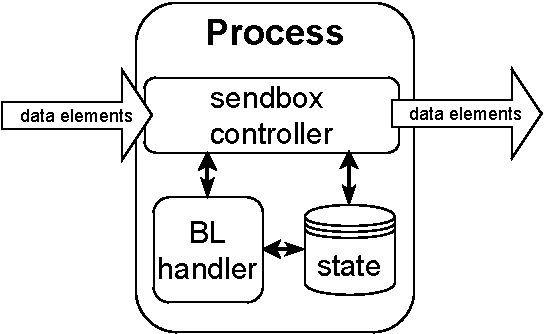
\includegraphics[width=0.25\textwidth]{pics/process-scheme.pdf}
  \caption{Structure of the SPE process}
  \label{fig:spe_process}
\end{figure}

Typically, distributed stream processing engines are shared-nothing runtimes that continuously ingest input elements, transform them according to a logical dataflow graph, and deliver output elements. The logical dataflow graph consists of user-defined operators. Operators can be stateless or stateful: an output element may depend on the current state and the corresponding input element. A logical graph is mapped to a physical, distributed graph on deployment. Commonly, a single logical operator can be deployed on multiple computational nodes. Further, we denote physical instances of logical operators as {\em processes}.

A deployed physical graph is a distributed system and could be described in terms of the Chandy-Lamport model~\cite{Chandy:1985:DSD:214451.214456, carbone2018scalable}. In this model, the authors introduce \textit{events} that allow observing a state of the entire system. This approach allows defining system-wide guaranties: in the original paper it is used to introduce notion of {\em consistent state}, we use this approach for definition of substream management problem.

Following notation from~\cite{Chandy:1985:DSD:214451.214456, carbone2018scalable}, each event is a tuple of 5 elements $e = (p, s, s', c, M)$, where $p$ is one of the deployed processes, $s$ and $s'$ are state of the process before and after processing, $c$ one of network FIFO channels that connect processes, and $M$ is a message generated during processing. The generated event $M$ comes to a channel state $C$ until the destination process receives it. Processes and channels form a physical graph of the system $G=\{\Pi,\mathcal{E}\}$. All incoming channels we denote as $I_p$ and output channels as $O_p$.

In a stream processing engine, we need to specify a process $p$ to reflect the specifics of this type of processing. In our model we split a process into two separate blocks: {\em business logic handler} (BLH), and {\em mailbox controller} (MBC). The first block encapsulates user-defined operator. In this scheme user-defined operator does not directly communicate with other processes in the system. Instead of this it receives and generates {\em messages} -- data elements that are tagged by their source and destination. Delivery of these messages along the communication channels is then proceed by mailbox controller. This system layout is not new and it is widely used in practise (Akka, YDB, Millwheel, etc.).

More formally, when a process receives a message it is handled by mailbox controller, that stores this message into a special segment of the process state ({\em mailbox} $B_p$). Business logic handler gets a message from the mailbox and triggers a user-defined operator. User-defined operator process the data element the message contains and generates arbitrary number of outgoing messages. BLH stores generated messages back to a mailbox. MBC iterate outgoing messages in the mailbox and send them along communication channels to destination processes. If user-defined operator have a state $U_p$, the joined process state will consist of the mailbox and this state $s=U_p \cup B_p$. In Chandy-Lamport paradigm this algorithm produce the following events within a process:
\begin{itemize}
    \item Communication events: $\langle recv, M\rangle$, $\langle send, M \rangle$ -- these events are handled by mailbox controller
    \item Processing of an incoming message $\langle proc, M\rangle$
\end{itemize}

Lets translate these events into 5-tuple language. Communication events moves a message between communication channel and mailbox section of the state:
\begin{eqnarray}
\langle recv, p, M\rangle = (p, s_p, s'_p = U_p \cup \left(B_p \cup \{M\}\right), c_{qp}, M) \\
\langle send, p, M \rangle = (p, s_p, s'_p = U_p \cup \left(B_p\setminus\{M\}\right), c_{p, dst(M)}, M)
\end{eqnarray}

Note that we need to be able to get a destination process directly from the message $dst(M)$. This function translates destination element from logical dataflow graph nodes, that are used in used-defined code, to physical communication channels between processes. A practical case of this abstraction is a sharding scheme for some key: user-defined procedure emits event for some key, and a system is responsible for finding a proper physical channel to deliver this message.

Incoming message processing does not influence the communication channels and only ingest results of a message processing $(U', M') = func_p(U, M)$:
\begin{equation}
    \langle proc, p, M\rangle = (p, s_p, s'_p = U'_p \cup \left(B_p \setminus \{M\} \cup M' \right) , \emptyset, \emptyset)
\end{equation}
Note, that in this case $M'$ may contain more than one message.

We assume that within the same process $p$ all events are totally ordered by a local causal order relation $<_p$: $e^{0}_p,e^{1}_p,...,e^{i}_p,...$. This assumption is naturally satisfied in single-thread environment. To effectively use multiple threads we can settle multiple process into a single node~\footnote{Actor systems are good practical example of such settlement}.

% Substream system events will be defined latter in the description of a particular implementation. Note that all events within the same process $p$ are totally ordered by a local causal order relation $<_p$: $e^{0}_p,e^{1}_p,...,e^{i}_p,...$. 
% Atomicity of the events and their sequential nature allows a system to build guarantees for processing and state management.

\subsection{Substream management events}
The processing of unbounded data sequences sometimes is difficult, and it is easier to solve an unlimited stream of small tasks than a single task for an unlimited stream of data. We use a condition on a data elements to limit the scope of a task. The data elements that satisfy a condition form a {\em substream}. The practical examples of substreams are: ``clicks received in time window $w$'', or ``requests from user 0x0321da83'', etc.

For each process we want to get the first and the last element of a substream. The first one could be found naturally when it emerges, but get ensure that the will be no more events of a substream could be problematic. To obtain the strict substream termination guarantee source must promise that no more messages from substream emerge, and the system must ensure that there are no substream messages inside the system. The first task requires contract with particular data sources and is out of scope of this paper, while discussed in the literature~\cite{awad2019adaptive}. Instead, we focus on the second task that is challenging due to distributed nature of the system and the lack of some common message lifetime limit. This problem becomes even more difficult with the introduction of cycles into dataflow. The problem here is that processes are not isolated from each other and substream message could move from one process to another. That is why we need to observe all in-flight messages in the system.

Formally, a substream can be defined via propositional formula $Pred(e)$ for any system event. We have to use system events as they are ordered inside each process and can define a border of a substream. Sometimes it is more practical to induce this predicate to messages ($pred(M)$) involved in processing: $Pred(e) = (e = \langle proc, p, M \rangle) \wedge pred(M)$.

In this paper we are interested in such $Pred(e)$, that has limited lifespan within a process and want to know when substream starts and terminates: $\forall p, \exists t_0^p, t_1^p: \exists e: e_{t_0^p} <_p e <_p e_{t_1^p}, Pred(e) \And \forall e': e_{t_1^p} <_p e', \neg Pred(e')$. Lets boil this formula down: for each process $p$ in the system there must be two event indices $t_0^p$ for substream start and $t_1^p$ for its termination, such that events satisfying $Pred$ must be between these indices. 

A substream management problem is to define a special mechanism that estimates substream bound for each process. In our system model, we need to define a system event that indicates the bound of a substream for a process. We call this termination event or end-of-substream event, this appropriate :
\begin{equation}
  \langle eoss, p, Pred \rangle = (p, B_p, B_p\cup eoss(Pred), \emptyset, \emptyset)  
\end{equation}

As we mentioned before, some problems require certain properties of the termination events. For example, the state pruning problem does not require any special properties, while for the state snapshotting problem, the substream management system should detect the exact substream bound. In the following sections, we formalize these properties. 

\subsubsection{Soft bound}

Many applications that apply substream management systems do not require any special properties of termination events. In this case, we denote the guarantee provided by such events as {\em soft bound}, because termination events indicate only the fact that the substream ended some time ago, and other input elements could be processed after that. More formally, we define the soft bound guarantee of the termination event (end-of-substream) $\langle eoss_{soft}, p, Pred\rangle$ as follows:

\begin{equation}
\forall e, e >_p \langle eoss_{soft}, p, Pred\rangle \Rightarrow \neg Pred(e)
\end{equation}

Figure~\ref{general_guarantees} illustrates this notion. Terms $a,b,c,d...$ denote ordered processing events of a process $p$. The substream ends after event $c$. Note that there are several other events between the end-of-substream and $c$. This is the property of a {\em soft bound} guarantee: if $\langle eoss_{soft}, p, Pred\rangle$ occurs, all subsequent elements do not satisfy the predicate, but it is not necessarily the exact substream ``border''.

\begin{figure}[htbp]
  \centering
  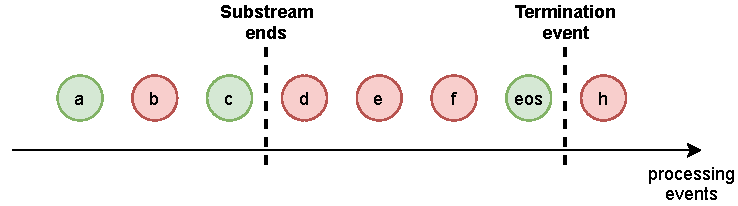
\includegraphics[width=0.50\textwidth]{pics/general-guarantee.pdf}
  \caption{Substream management: soft bound}
  \label{general_guarantees}
\end{figure}

\subsubsection{Firm bound}

The guarantee that any new event will not satisfy the predicate is sufficient for many real-life problems, e.g., SPE can initiate process state pruning on such events. However, some problems require a {\em firm bound}: guarantee that the substream ends {\em exactly} after the termination event. 

For example, epoch-based snapshotting protocol~\cite{2015arXiv150608603C, jacques2016consistent} bases on a notion of {\em epoch}. Epoch is a special substream that should be atomically processed. Therefore, SPE requires the termination event for an epoch that occurs right after the last processing event for this epoch. Otherwise, the snapshot can be inconsistent, because it captures elements from various epochs. To support such scenarios, the end-of-substream event $\langle eoss_{firm}, p, Pred\rangle$ should satsify the following condition:

\begin{equation}\begin{array}{l}
\langle eoss_{firm}, p, Pred\rangle = \inf_{p} \langle eoss_{soft}, p, Pred\rangle
\end{array}\end{equation}

Unlike soft bound the firm one guarantee that the first element outside the substream $Pred$ must be ordered after the firm bound event in the process $p$. This position satisfies to the first possible soft bound in the events ordering. Figure~\ref{strict_guarantees} illustrates the notion of the firm bound. As in the previous example, terms $a,b,c,d...$ denote ordered processing events of a process $p$. However, in this case, event $\langle eoss_{firm}, p, Pred\rangle$ occurs right after the substream terminates.

\begin{figure}[htbp]
  \centering
  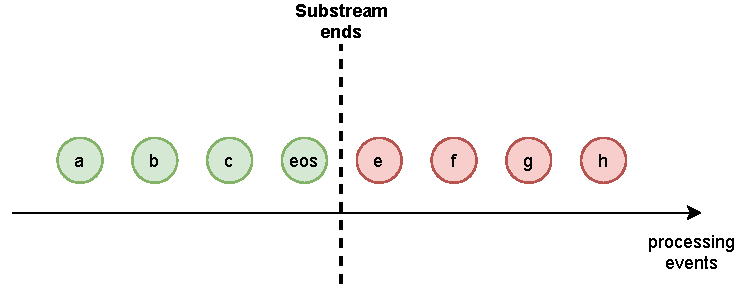
\includegraphics[width=0.50\textwidth]{pics/strict-guarantee.pdf}
  \caption{Substream management: firm bound}
  \label{strict_guarantees}
\end{figure}

\subsubsection{Consistent termination events order}
Some specific applications, including the mentioned earlier epoch-based snapshotting method and techniques for enforcing deterministic processing~\cite{we2018adbis} require an order of termination events to be synchronized with the order of substreams endings (events from data sources). For example, if termination events are reordered, then snapshots for consecutive epochs can be inconsistent. Another example is deterministic join that also requires the defined order of termination events~\cite{gulisano2016scalejoin}.

\begin{figure}[htbp]
  \centering
  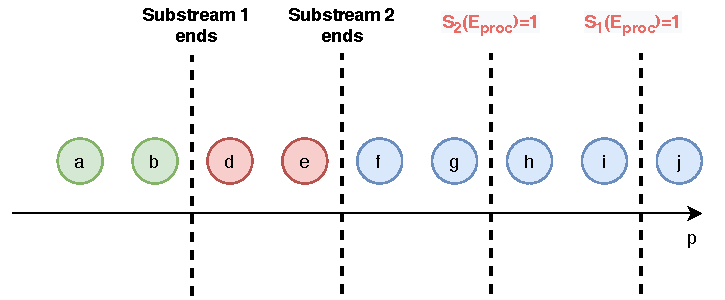
\includegraphics[width=0.50\textwidth]{pics/notifications-reordering.pdf}
  \caption{An example of termination events reordering}
  \label{notifications_reordering}
\end{figure}

Termination events reordering in case of the soft bound guarantee is illustrated in Figure~\ref{notifications_reordering}. Terms $a,b,c,d...$ denote ordered processing events of a process $p$. Although the substream containing events $a,b$ terminates earlier, the end-of-substream event for this substream occurs after the termination event for the substream containing events $d,e$. 

Let $e^{*}_1$ and $e^{*}_2$ be the last elements of substreams defined by predicates $pred_1(m)$ and $pred_2(m)$. Termination events $\langle eoss, p, pred_1(m)\rangle$ and $\langle eoss, p,  pred_2(m)\rangle$ are {\em consistently ordered} iff:

\begin{equation}
e^{*}_1 >_p e^{*}_2 \Leftrightarrow \langle eoss, pred_1(m)\rangle >_p \langle eoss, pred_2(m)\rangle
\end{equation}

\subsubsection{Optimal traffic overhead}

A vital performance property of a substream management system is the amount of extra network traffic. Let $|\Pi|$ be a number of processes, and $K$ be a number of substreams. 

\begin{lemma}
The network overhead induced by a substream management system cannot be lower than $O(K|\Pi|)$. 
\end{lemma}
\begin{proof}
When a substream management system detects the end of a substream, each stateful process should be informed about this. In a general case, e.g., for a state snapshotting problem, it should inform all processes. Hence, at least one network message (termination notification) must be received by each process for each substream.
\end{proof}

Despite this lemma's simplicity, we will further use it to figure out how far is some substream management system from this bound. We can also claim a solution as {\em optimal} if its extra traffic estimation is equal to the lower bound from the lemma. In the next sections, we demonstrate that it is possible to design a substream management system that achieves optimal network traffic overhead.

\subsection{Punctuations framework}
\label{fs-acker-punctuations}

The main idea behind the punctuations framework is to inject special data elements $\mathcal{P}^{pred}$ into data stream one per substream. These elements, called punctuations, flows down the workflow as ordinary data elements. The injector promises that all elements after punctuations won't satisfy the predicate. Hence, the punctuation itself defines the ``border'' of a substream.

Figure~\ref{punctuations_scheme} illustrates the punctuations framework. Green elements indicate elements that belong to some substream, while red elements do not. As we can see, punctuations play the role of delimiter between the substream elements and all further items.

\begin{figure}[htbp]
  \centering
  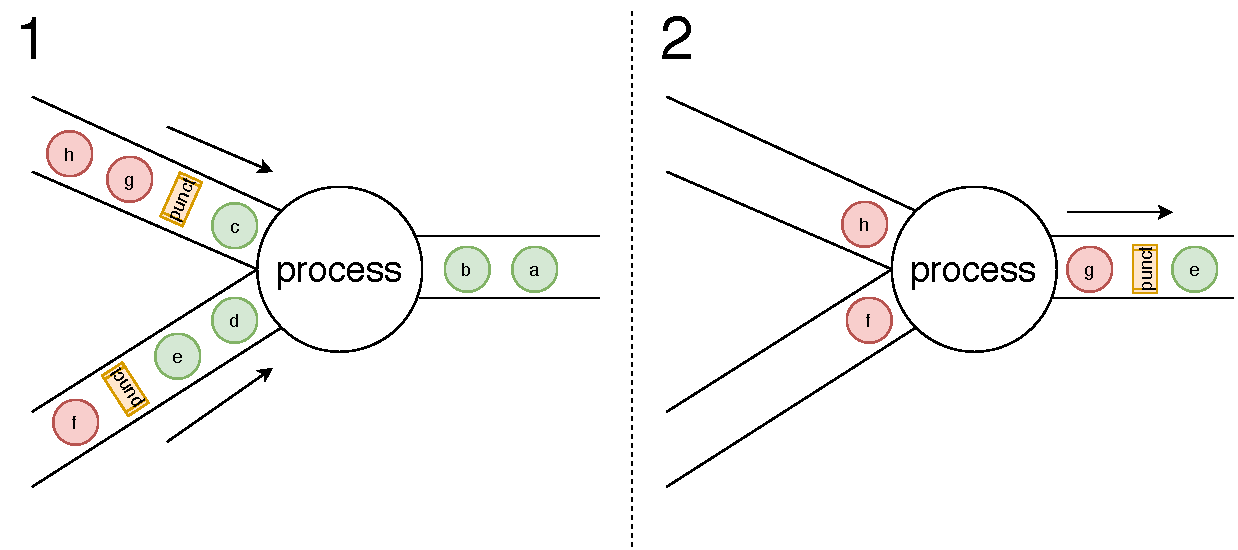
\includegraphics[width=0.50\textwidth]{pics/punctuations-scheme.pdf}
  \caption{Punctuations framework: an example}
  \label{punctuations_scheme}
\end{figure}

Processes within SPE do not apply user-defined operators to punctuations. Instead, each process $p$ propagates punctuation data element to all outgoing channels $c_{pq} \in O_p$ in messages $\mathcal{P}_{pq}^{pred}$ when it receives corresponding punctuations from all input channels $I_p$. If a process receives punctuations from all inputs, it is guaranteed that it will not receive elements that satisfy the predicate further due to FIFO network channels. It in easy to show that generating event by following rule make it a soft bound of the substream $pred$:
\begin{equation}
\forall q \in I_p, \exists \mathcal{P}^{pred}_{qp} \in B_p, \forall M\in B : \neg pred(M) \wedge dst(M) \ne p
\end{equation}

Note, that we must ensure that mailbox does not contain incoming messages of the substream ($pred(M) \wedge dst(M) = p$) before claiming soft bound.

To satisfy the firm bound guarantee, one needs to hold elements in the mailbox until all punctuations have arrived from all input channels. In~\cite{Carbone:2017:SMA:3137765.3137777} such behavior is called {\em watermark (punctuation) alignment}. More formally, the mailbox procedure should ensure the following order of elements processing to achieve firm bound:

\begin{align*}
& \exists q \in I_p, e = \langle recv,m_{qp} \rangle >_p e^{'} = \langle recv,punct_{qp}\rangle \Longrightarrow \\ 
& \langle proc, m_{qp}\rangle >_p \langle eoss_{soft}, pred(m)\rangle
\end{align*}

If this condition is satisfied, then $\langle eoss_{firm}, pred(m)\rangle$ = $\langle eoss_{soft}, pred(m)\rangle$ for the punctuations. The punctuations framework provides consistent termination events order by design because punctuations are naturally ordered with ordinary data elements within the processes.

While the punctuations approach is robust and easy-to-implement, it has several limitations. In the punctuations framework, the information about the ending of a substream is propagated using ordinary data elements via the data flow network channels. It implies that punctuations are not applicable for cyclic dataflows because a process that receives elements from a cyclic channel will never receive punctuations from this channel~\cite{carbone2018scalable}.

The high network overhead forms another limitation. This method's amount of service traffic is $O(K|\Pi|^2)$, where $|\Pi|$ is the number of processes and $K$ is the number of substreams. As we can see, this estimation is far from the lower bound ($O(|\Pi|)$). It is quadratic in the number of processes, as each process should propagate punctuations to all output channels. 

Substreams can be {\em fine-grained}: for example, each user session defines a substream. If there are a lot of small substreams, an inefficient substream management system can reduce the throughput of an SPE itself~\cite{Li:2008:OPN:1453856.1453890} or affect the performance of state checkpointing~\cite{zhang2021research}. As we demonstrate further, the punctuation technique adds significant performance overhead on regular processing for small substreams (frequent punctuations injection).